\documentclass[11pt,letterpaper]{article}
\usepackage[margin=1in]{geometry}
\usepackage{amsmath,amssymb,amsthm,mathtools}
\usepackage{microtype}
\usepackage{booktabs}
\usepackage{xcolor}
\usepackage{graphicx}
\usepackage{tikz}
\usetikzlibrary{positioning,arrows.meta}
\definecolor{focalteal}{HTML}{1F6F5F}
\definecolor{risktone}{HTML}{B5473C}
\usepackage{enumitem}
\usepackage[hidelinks]{hyperref}
\usepackage[nameinlink,capitalise,noabbrev]{cleveref}

\newtheorem{definition}{Definition}
\newtheorem{theorem}{Theorem}
\newtheorem{proposition}{Proposition}
\newtheorem{lemma}{Lemma}
\newtheorem{corollary}{Corollary}
\newtheorem{remark}{Remark}
\newtheorem{conjecture}{Conjecture}

\newcommand{\X}{\mathcal{X}}
\newcommand{\Y}{\mathcal{Y}}
\newcommand{\Impact}{C_{\Delta}}
\newcommand{\ImpEdges}{E_{\Delta}}
\newcommand{\E}{\mathbb{E}}
\newcommand{\Prb}{\mathbb{P}}
\newcommand{\KL}{\mathrm{KL}}
\newcommand{\kl}{\mathrm{kl}}
\newcommand{\PsiG}{\Psi}

\title{\textbf{Testing Fairness of Evolving Software under Uncertainty}}
\author{Author name(s) and affiliation(s) to be finalized}
\date{}

\begin{document}
\maketitle

\begin{abstract}
Software fairness is usually audited as if a program were a fixed deterministic
object.  Real software evolves through patches and can be stochastic because of
randomized logic, scheduling, concurrency, resource contention, and environmental
state.  We study \emph{fairness regression testing}: after a previously certified
program is modified, how many executions are fundamentally necessary to determine
whether the patch has introduced a fairness violation?

We model valid counterfactual comparisons by a graph whose vertices are software
inputs and whose edges identify pairs that should receive sufficiently similar
outcomes.  A patch is accompanied by a sound change-impact region.  Regression
testing additionally exposes two executable program versions.  We therefore study
a \emph{coupled differential execution oracle}: the old and new versions are run
on the same input under a shared random tape, allowing the tester to estimate the
patch-induced behavioral delta directly.

For a Gaussian core problem, we identify an uncertainty-weighted graph quantity
$\Psi(H,\nu)$ that captures how executions should be shared across counterfactual
comparisons.  A non-adaptive tester has complexity
$O(\Psi(H,\nu)\gamma^{-2}\log(|E(H)|/\delta))$, while every adaptive
$\delta$-correct tester requires
$\Omega(\Psi(H,\nu)\gamma^{-2}\log(1/\delta))$ expected paired-oracle calls on a
null instance.  Sound patch localization yields a linear separation on a matching
family.  For Bernoulli software, we further distinguish ordinary old/new pairing
from \emph{four-way counterfactual replay}, which synchronizes the random tape
across both software versions and both endpoints of a fairness edge.  When a patch
has a nonzero fairness-neutral common effect $s$ and a smaller differential
fairness effect $d$, four-way replay cancels the common effect pathwise and has
$\Theta(d^{-1}\log(1/\delta))$ fixed-confidence complexity, whereas
vertex-paired replay requires
$\Theta(d^{-2}\log(1/\delta))$ calls for fixed interior $s$.  Under the stronger
synchronized-suite replay primitive, one shared random tape is applied to both
versions at every fairness-active input.  In the corresponding homogeneous
Bernoulli family, all fairness edges are tested simultaneously: round complexity
is $\Theta(d^{-1}\log(1/\delta))$ and concrete execution complexity is
$\Theta(n_+d^{-1}\log(1/\delta))$, independent of the number of fairness edges.
For intermediate \emph{partial replay}, where only declared input groups may
share randomness, we identify two fractional-cover geometries.  Four-way
edge-witness scheduling can be arbitrarily more expensive, or even infeasible,
while the raw-output information geometry is an active-vertex cover
$C_{\rm vert}$.  In the frozen homogeneous single-changed-endpoint family, a
within-group patch-delta contrast test attains this same $C_{\rm vert}$ geometry,
giving matching lower/upper combinatorial dependence and
$\Theta(d^{-1}\log(1/\delta))$ fixed-confidence order up to constants and
rounding.  Thus version-aware replay can change both the small-effect exponent
and the graph geometry of fairness-regression testing.

These results establish a tractable foundation for the broader objective of tight
query complexity for fairness regression with retained certificates, heterogeneous
uncertainty, imperfect change-impact information, and multiple software versions.
\end{abstract}

\section{Introduction}
\label{sec:intro}

Software evolves continuously.  Regression testing is therefore not a secondary
engineering convenience: it is the mechanism by which evidence about an earlier
version is reused to decide whether a modified version still satisfies its
requirements.  Classical regression-test selection and change-impact analysis
make this reuse explicit \cite{RothermelHarrold1996,YooHarman2012,LiSunLeungZhang2013},
and recent incremental-verification work similarly reuses proof artifacts across
program versions \cite{YinEtAl2025}.

Fairness creates a regression requirement with an additional statistical
challenge.  Software fairness testing is established as a testing problem
\cite{GalhotraBrunMeliou2017}, while online fairness auditing studies how observations can be adaptively allocated
to assess a fixed deployed system \cite{ManerikerBurleyParthasarathy2023}.  Yet
software may itself be nondeterministic even in the complete absence of learned
models.  Randomized tie-breaking, task scheduling, concurrent interleavings,
resource contention, random backoff, clocks, and other nondeterministic APIs can
make repeated executions of the same code and input disagree.  Recent testing
work continues to find nondeterminism central to flakiness \cite{YuanLinShi2026}.

We ask a version-aware question:
\begin{quote}
\emph{Given a previously certified program, a patch, and stochastic execution
access to the old and new versions, what is the minimum number of executions
required to detect or rule out a fairness regression?}
\end{quote}

The regression setting contributes two pieces of information absent from fresh
auditing.  First, a sound change-impact analysis can localize where behavior may
have changed.  Second, the old version remains executable.  If stochastic choices
can be replayed through a controlled seed or random tape, $P_0$ and $P_1$ can be
run under the same execution randomness.  Their difference then estimates the
patch itself.  This is related to the classical common-random-numbers principle in
simulation \cite{GlassermanYao1992}, and to coupling as a formal technique for
reasoning about pairs of probabilistic programs \cite{BartheEtAl2017}; our use is
as an information model for regression testing.

We represent fairness requirements by a counterfactual graph $G=(V,E)$.  A vertex
is a valid software input and an edge is a pair whose expected outcomes should
remain sufficiently close.  A patch produces expected behavioral changes
$\theta_v=\mu_{1,v}-\mu_{0,v}$.  The central core problem asks whether
$\theta_u=\theta_v$ on every impacted fairness edge or whether at least one edge
has differential patch effect at least $\gamma$.  This \emph{patch-neutrality}
problem is stronger than full thresholded fairness preservation but isolates the
information-theoretic interaction among version reuse, graph structure, and
stochastic execution.

For Gaussian paired deltas we derive a graph complexity
\[
\Psi(H,\nu)=
\min_{q_v>0}\left\{
\sum_v q_v:
\frac{\nu_u^2}{q_u}+\frac{\nu_v^2}{q_v}\le1
\ \forall (u,v)\in E(H)
\right\},
\]
where $\nu_v^2$ is the variance of the old--new behavioral difference at vertex
$v$.  A static allocation based on $\Psi$ gives the upper bound, while an adaptive
change-of-measure argument gives a matching dependence on $\Psi$ and
$\gamma^{-2}$ in the lower bound.  We also derive the Lagrange dual, making clear
that the same executions can support several incident counterfactual comparisons.

The regression advantage appears directly in the variance.  If $Y_0,Y_1$ are old
and new outcomes produced under the same random tape,
\[
\mathrm{Var}(Y_1-Y_0)
=
\mathrm{Var}(Y_1)+\mathrm{Var}(Y_0)-2\mathrm{Cov}(Y_1,Y_0).
\]
When nearby versions respond similarly to the same stochastic environment, the
covariance can be large and the patch can be substantially easier to estimate
than either absolute program behavior.  In a common-uniform Bernoulli model, a
change from success probability $p$ to $p+d$ yields differential variance
$d(1-d)$, which vanishes with patch size even when the marginal outcome variances
remain bounded away from zero.


Our Bernoulli results expose a second form of reuse.  Four-way counterfactual
replay synchronizes randomness across the old and new versions and both endpoints
of one fairness edge.  A fairness-neutral common patch effect then cancels
pathwise, while a differential effect of size \(d\) remains a sparse witness;
this changes fixed-confidence complexity from quadratic to linear in \(1/d\).
If the test harness can replay one seed across the entire fairness-active input
suite, the same round simultaneously exposes every counterfactual edge.  For the
homogeneous family analyzed in \Cref{thm:suite-replay}, the number of replay
rounds is independent of \(|E|\), and concrete execution complexity scales with
the number of active inputs rather than the number of fairness comparisons.
This stronger oracle is stated explicitly: it is not assumed available to every
software system.

Between edgewise replay and full-suite replay lies a partial-replay regime in
which only declared groups of inputs can share a tape.  Here two combinatorial
objects diverge.  A four-way edge witness requires a replay group containing both
fairness endpoints, whereas raw transcript information requires only the changed
active endpoint plus a synchronized reference.  We show that the corresponding
edge-cover geometry can exceed the active-vertex cover $C_{\rm vert}$ by an
unbounded factor and can even be infeasible.  More importantly, for the frozen
homogeneous single-changed-endpoint Bernoulli family, the raw information is
operational: scheduling groups by $C_{\rm vert}$ and rejecting on a nonconstant
within-group vector of old--new patch deltas yields zero type-I error and
$O(C_{\rm vert}d^{-1}\log(1/\delta))$ fixed-design cost, while transcript
change of measure gives the matching $C_{\rm vert}$ combinatorial lower
geometry.  This theorem is deliberately not extended to heterogeneous
fairness-preserving nulls, where unrelated synchronized references can undergo
different benign patch effects.

The paper is deliberately theory-first and model-free.  No pretrained model,
open-source model, proprietary API, or LLM is an experimental subject.  GPU
computation is used only to falsify conjectures, validate implementations, and
stress-test the proved complexity laws on large synthetic instances.

\begin{figure}[t]
\centering
\resizebox{\textwidth}{!}{%
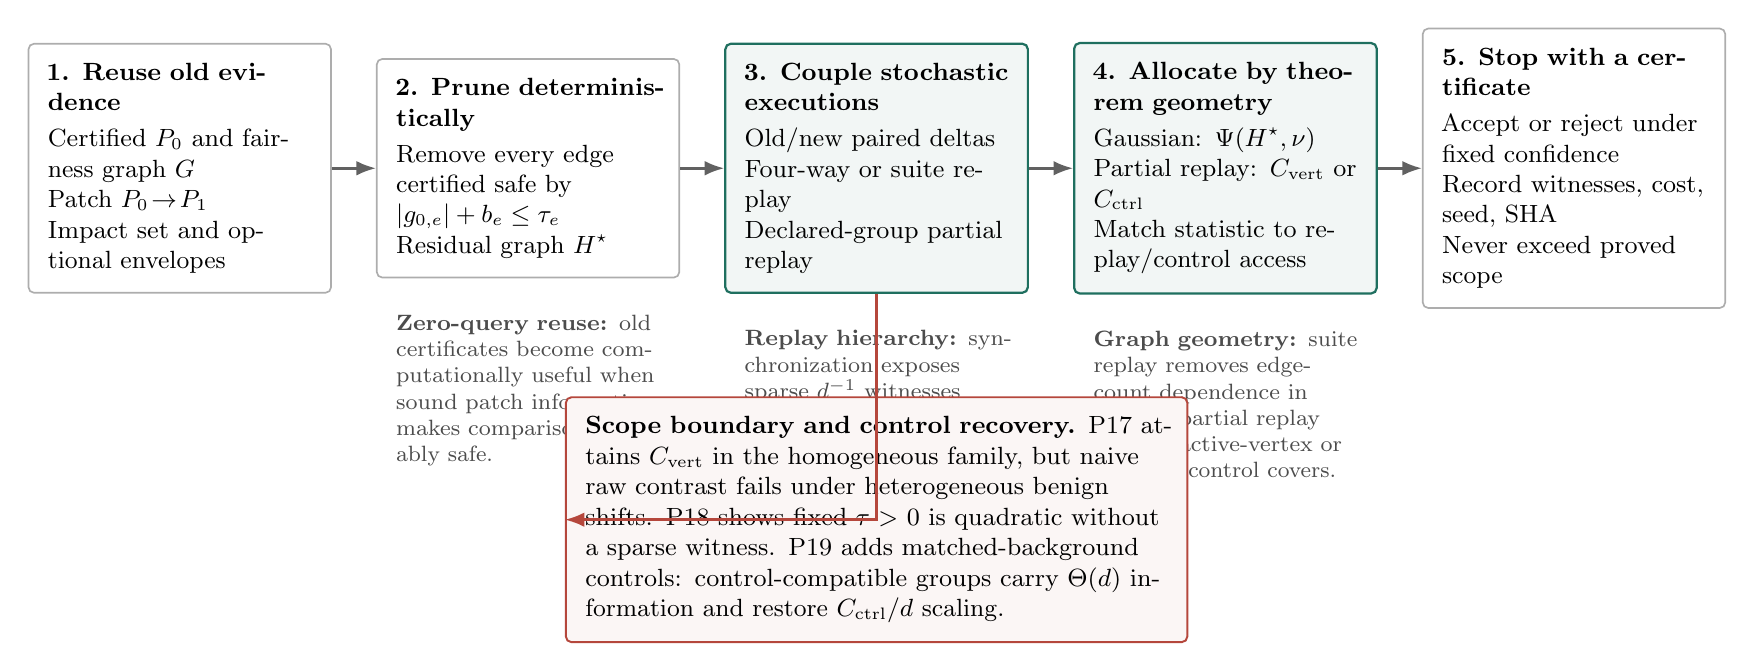
\begin{tikzpicture}[
  >=Latex,
  node distance=0.62cm and 0.56cm,
  stage/.style={draw=black!32, rounded corners=2pt, line width=0.6pt,
               fill=white, minimum height=1.65cm, text width=3.35cm,
               align=left, inner sep=7pt, font=\small},
  focal/.style={stage, draw=focalteal, line width=0.8pt, fill=focalteal!6},
  risk/.style={stage, draw=risktone, line width=0.7pt, fill=risktone!5},
  flow/.style={->, line width=0.9pt, draw=black!62},
  sub/.style={font=\footnotesize, text=black!70, align=left}
]

\node[stage] (inputs) {
  \textbf{1. Reuse old evidence}\\[2pt]
  Certified $P_0$ and fairness graph $G$\\
  Patch $P_0\!\to\!P_1$\\
  Impact set and optional envelopes
};

\node[stage, right=of inputs] (prune) {
  \textbf{2. Prune deterministically}\\[2pt]
  Remove every edge certified safe by\\
  $|g_{0,e}|+b_e\le\tau_e$\\
  Residual graph $H^\star$
};

\node[focal, right=of prune] (observe) {
  \textbf{3. Couple stochastic executions}\\[2pt]
  Old/new paired deltas\\
  Four-way or suite replay\\
  Declared-group partial replay
};

\node[focal, right=of observe] (allocate) {
  \textbf{4. Allocate by theorem geometry}\\[2pt]
  Gaussian: $\Psi(H^\star,\nu)$\\
  Partial replay: $C_{\rm vert}$ or $C_{\rm ctrl}$\\
  Match statistic to replay/control access
};

\node[stage, right=of allocate] (decision) {
  \textbf{5. Stop with a certificate}\\[2pt]
  Accept or reject under fixed confidence\\
  Record witnesses, cost, seed, SHA\\
  Never exceed proved scope
};

\draw[flow] (inputs) -- (prune);
\draw[flow] (prune) -- (observe);
\draw[flow] (observe) -- (allocate);
\draw[flow] (allocate) -- (decision);

\node[sub, below=0.34cm of prune, text width=3.35cm] (zero) {
  \textbf{Zero-query reuse:} old certificates become computationally useful
  when sound patch information makes comparisons provably safe.
};

\node[sub, below=0.34cm of observe, text width=3.35cm] (replay) {
  \textbf{Replay hierarchy:} synchronization exposes sparse $d^{-1}$ witnesses
  directly, or recovers them through matched-background controls.
};

\node[sub, below=0.34cm of allocate, text width=3.35cm] (geometry) {
  \textbf{Graph geometry:} suite replay removes edge-count dependence in
  rounds; partial replay induces active-vertex or matched-control covers.
};

\node[risk, below=1.30cm of observe, text width=7.40cm] (scope) {
  \textbf{Scope boundary and control recovery.} P17 attains $C_{\rm vert}$
  in the homogeneous family, but naive raw contrast fails under heterogeneous
  benign shifts. P18 shows fixed $\tau>0$ is quadratic without a sparse
  witness. P19 adds matched-background controls: control-compatible groups carry
  $\Theta(d)$ information and restore $C_{\rm ctrl}/d$ scaling.
};

\draw[flow, draw=risktone] (observe.south) |- (scope.west);

\end{tikzpicture}%
}
\caption{TFOESUU overview.  Fairness regression is treated as evidence reuse
across software versions: deterministic change information first removes
comparisons that need no new executions; the remaining stochastic problem is
matched to the strongest sound replay primitive; theorem-specific allocation
then controls execution cost.  The red box combines the P17 scope obstruction,
P18's threshold phase boundary, and P19's matched-control recovery, making clear
that replay strength alone is insufficient: the topology of valid synchronized
controls can change both the exponent and the governing fractional geometry.}
\label{fig:overview}
\end{figure}
\begin{table}[t]
\centering
\caption{Main complexity results at a glance.  Orders suppress universal constants;
$\delta$ is the target error probability.  Rows state proved scope only.}
\label{tab:main-results}
\small
\begin{tabular}{@{}p{0.22\textwidth}p{0.23\textwidth}p{0.27\textwidth}p{0.15\textwidth}@{}}
\toprule
Setting & Reused information / access & Fixed-confidence cost & Status \\
\midrule
Gaussian patch neutrality & Old/new paired deltas on residual graph $H$ &
$\Theta(\Psi(H,\nu)\gamma^{-2}\log(1/\delta))$ up to the upper-bound
$\log |E(H)|$ factor & Proved + audited \\

Patch-localized matching & Sound impact location & Removes the $M$-edge
location-search factor on the matching family & Proved + audited \\

Bernoulli one-edge replay & Common-uniform old/new pairing &
$\Theta(d^{-1}\log(1/\delta))$ versus $\Theta(d^{-2}\log(1/\delta))$
for fresh/independent sampling at fixed interior $p$ & Proved + audited \\

Four-way counterfactual replay & One tape across both versions and both
fairness endpoints & $\Theta(d^{-1}\log(1/\delta))$ versus vertex-paired
$\Theta(d^{-2}\log(1/\delta))$ with nonzero common patch effect & Proved + audited \\

Thresholded one-edge replay & Four-way synchronized replay with fairness tolerance $\tau$ &
$\Theta((\tau+d)d^{-2}\log(1/\delta))$; $\tau=O(d)$ gives $d^{-1}$ while fixed $\tau>0$ gives $d^{-2}$ &
Proved + audited \\

Synchronized-suite replay & One tape across all fairness-active inputs &
Rounds $\Theta(d^{-1}\log(1/\delta))$; executions
$\Theta(n_+d^{-1}\log(1/\delta))$, independent of edge count in the
homogeneous family & Proved + audited \\

Partial synchronized replay & Declared replay groups &
$C_{\rm vert}d^{-1}\log(1/\delta)$ combinatorial geometry up to constants
and rounding in the frozen homogeneous single-changed-endpoint family &
Proved + audited in stated scope \\
\bottomrule
\end{tabular}
\end{table}
\section{Model}
\label{sec:model}

\subsection{Random-tape software semantics}
Let $\X$ be a finite domain of valid software inputs, $\mathcal{R}$ a random-tape
space, and $\Y\subseteq\mathbb{R}$ an outcome space.  Version $P_j$,
$j\in\{0,1\}$, is a measurable map
\[
P_j:\X\times\mathcal{R}\to\Y.
\]
An execution on input $x$ draws $R\sim\mathcal{R}_x$ and returns $P_j(x;R)$.
Define
\[
\mu_{j,x}=\E[P_j(x;R)],
\qquad
\sigma_{j,x}^2=\mathrm{Var}(P_j(x;R)).
\]
Deterministic software is the special case in which the output does not depend on
$R$.

\subsection{Counterfactual fairness graph}
Let $G=(V,E)$ with $V\subseteq\X$.  An edge $e=(u,v)$ encodes a valid
counterfactual comparison.  For scalar expected outcomes we require
\[
|\mu_{j,u}-\mu_{j,v}|\le\tau_e.
\]

\begin{definition}[Fairness on $G$]
Version $P_j$ is fair on $G$ if the inequality above holds for every edge in $E$.
\end{definition}

\subsection{Patch and impact information}
A patch $\Delta$ maps $P_0$ to $P_1$.  A change-impact analysis returns
$\Impact\subseteq V$.

\begin{definition}[Distributionally sound impact set]
$\Impact$ is distributionally sound if
\[
x\notin\Impact\implies P_0(x;R)\overset{d}=P_1(x;R).
\]
\end{definition}

\begin{definition}[Replay-sound impact set]
$\Impact$ is replay-sound if
\[
x\notin\Impact\implies P_0(x;R)=P_1(x;R)
\quad\text{almost surely under shared replay.}
\]
\end{definition}

Define
\[
\ImpEdges=\{(u,v)\in E:u\in\Impact\text{ or }v\in\Impact\},
\]
and let $H$ contain exactly the vertices incident to $\ImpEdges$ and the impacted
edges among them.

\subsection{Patch effects}
Define
\[
\theta_v=\mu_{1,v}-\mu_{0,v}.
\]
For edge $e=(u,v)$, if $g_{j,e}=\mu_{j,u}-\mu_{j,v}$, then
\[
g_{1,e}=g_{0,e}+(\theta_u-\theta_v).
\]
The identity separates previously certified behavior from the effect of the patch.

\section{Algorithmic Framework}
\label{sec:algorithm}

The theory induces an executable regression-testing procedure rather than a
single monolithic statistical test. The tester first reuses deterministic
software-evolution information, enumerates the replay observations the harness
can actually implement, and selects a theorem-backed test whose assumptions
match the residual problem. Stronger synchronization per round need not imply
lower concrete execution cost.

\begin{figure}[t]
\centering
\setlength{\fboxsep}{8pt}
\colorbox{black!5}{\begin{minipage}{0.93\textwidth}
\textbf{Algorithm 1: TFOESUU fairness-regression tester}

\smallskip
\textbf{Input:} certified old program $P_0$, patched program $P_1$, fairness
graph $G=(V,E)$, thresholds $\{\tau_e\}$, confidence $\delta$, sound impact
information, optional patch-effect envelopes $\{b_e\}$, and an executable
replay capability.

\begin{enumerate}[leftmargin=1.6em,itemsep=2pt,topsep=3pt]
\item \textbf{Prune by deterministic evidence.}
Remove every edge $e$ whose certificate and sound envelope imply
$|g_{0,e}|+b_e\le \tau_e$.  Let the remaining graph be $H^\star$.

\item \textbf{Stop if nothing remains.}
If $E(H^\star)=\varnothing$, return \textsc{Accept} with zero additional
stochastic executions.

\item \textbf{Determine admissible replay actions and costs.}
Record which inputs and versions can share one random tape: old/new vertex
pairs, four-way edges, declared partial-replay groups, or a complete active
suite. For each implementable action record both its observation law and
its cost in concrete program executions. Do not assume a total cost ordering
among these primitives: a suite query observes more but also executes more
configurations.

\item \textbf{Select a scoped statistical plan and allocate calls.}
For the Gaussian paired-delta core, use $\Psi(H^\star,\nu)$ only under its
stated variance and margin assumptions. For homogeneous partial replay use
$C_{\rm vert}$; for the audited two-class matched-control family use
$C_{\rm ctrl}$ only when its control compatibility assumptions hold.
Use the corresponding finite-confidence sampling construction for eligible
four-way, thresholded, or suite replay. Compare cost bounds only after
converting them to consistent execution units. Otherwise decline to
certify rather than extrapolate from an inapplicable theorem.

\item \textbf{Evaluate only a test justified by the selected model.}
Estimate paired patch contrasts or use the synchronized witness prescribed by
the chosen theorem. The homogeneous within-group nonconstant-delta predicate
is valid only under its frozen null; P19 requires matched-background controls.
The candidate P20 composite-nuisance information LP is not a certified
testing algorithm or stopping rule.

\item \textbf{Return a scope-qualified fixed-confidence decision.}
Return \textsc{Reject} with the test evidence when its rejection condition
fires, or \textsc{Accept} only once the selected model's stipulated
fixed-confidence rule has been satisfied. Record tested null/alternative,
error target, replay groups, concrete executions, seeds, assumptions, and
source commit. Statistical acceptance is not a deterministic proof outside
the stated hypothesis family.
\end{enumerate}

\textbf{Guarantee discipline.}  The procedure inherits only the guarantee of
the selected proved theorem.  In particular, the P17 $C_{\rm vert}$
attainability result is restricted to the frozen homogeneous
single-changed-endpoint family.
\end{minipage}}
\caption{Executable high-level TFOESUU procedure.  The key design rule is to reuse deterministic certificates before sampling,
then select a legally replayable, theorem-compatible test with explicit
execution-cost accounting. Stronger replay access is not automatically cheaper
in concrete executions.}
\label{alg:tfoesuu}
\end{figure}
\paragraph{Executable correspondence.}
The repository implements this theorem-to-plan layer in
\path{src/tfoesuu/planner.py}.  The planner is intentionally fail-closed:
the P12 and P15 modes reject multi-edge requests, and the P17 mode requires an
explicit homogeneous single-changed-endpoint scope acknowledgement before it
will construct the active-vertex schedule.  Thus the software interface cannot
silently promote a theorem beyond the proof ledger.


\section{Localization and Statistical Separation}
\label{sec:localization}

\begin{proposition}[Localization of new violations]
\label{prop:localization}
If $P_0$ is fair on $G$ and $\Impact$ is distributionally sound, every fairness
violation newly introduced by $P_1$ lies in $\ImpEdges$.
\end{proposition}

\begin{proof}
For $e=(u,v)\notin\ImpEdges$, both endpoints lie outside $\Impact$.  Soundness
implies that both endpoint output distributions, and therefore both expectations,
are unchanged.  Hence $g_{1,e}=g_{0,e}$, and the previous fairness certificate for
$P_0$ remains valid on $e$.
\end{proof}

A stochastic tester cannot in general distinguish an exact threshold from an
arbitrarily small violation with a uniform finite query bound.

\begin{proposition}[No finite uniform sharp-threshold test]
\label{prop:zero-margin}
Fix $\tau\in(0,1/2)$ and $\delta\in(0,1/2)$.  On a graph containing one edge with
Bernoulli outputs, there is no tester with finite worst-case query bound that
uniformly distinguishes
\[
|p_u-p_v|\le\tau
\quad\text{from}\quad
|p_u-p_v|>\tau
\]
with success probability at least $1-\delta$ on every instance.
\end{proposition}

\begin{proof}
Take a fair instance on the boundary, e.g. $p_u=1/4$ and
$p_v=1/4+\tau$, and compare it with an unfair instance obtained by replacing
$p_v$ by $p_v+\eta$.  For any fixed finite query budget, the KL divergence between
the two possible transcript distributions tends to zero as $\eta\to0$.  Pinsker's
inequality therefore makes their total-variation distance arbitrarily small, so
no decision rule can maintain error at most $\delta$ in both worlds.
\end{proof}

Accordingly, the core problem uses a positive separation margin $\gamma>0$.

\section{Coupled Differential Execution}
\label{sec:coupled}

A coupled query to vertex $v$ draws one random tape $R$ and evaluates both
versions:
\[
Y_{0,v}=P_0(v;R),\qquad Y_{1,v}=P_1(v;R),
\]
returning
\[
Z_v=Y_{1,v}-Y_{0,v}.
\]
Then $\E[Z_v]=\theta_v$.  Write $\nu_v^2=\mathrm{Var}(Z_v)$.

\begin{proposition}[Differential variance]
\label{prop:diffvar}
\[
\nu_v^2
=
\sigma_{1,v}^2+\sigma_{0,v}^2
-2\mathrm{Cov}(P_1(v;R),P_0(v;R)).
\]
If the two versions instead use independent random tapes, the variance of their
difference is $\widetilde\nu_v^2=\sigma_{1,v}^2+\sigma_{0,v}^2$.
\end{proposition}

\begin{proof}
Expand the variance of $Y_{1,v}-Y_{0,v}$.  Under independent replay the covariance
term vanishes.
\end{proof}

\begin{corollary}[Equal-variance correlation gain]
If both versions have variance $\sigma^2$ and correlation $\rho$ at every relevant
vertex, then
\[
\nu_v^2=2\sigma^2(1-\rho),
\qquad
\widetilde\nu_v^2=2\sigma^2.
\]
Thus every query bound homogeneous of degree one in the vertex variances improves
by factor $1-\rho$ under paired replay.
\end{corollary}

Common random numbers are not universally beneficial \cite{GlassermanYao1992}.
The access model therefore exposes the actual paired-delta variance rather than
assuming positive correlation by fiat.

\section{A Gaussian Core Characterization}
\label{sec:gaussian}

Suppose a paired-oracle call to $v\in V(H)$ returns
\[
Z_v\sim\mathcal{N}(\theta_v,\nu_v^2),
\]
independently across paired-oracle calls, with known $\nu_v^2>0$.  We test
\[
\mathsf H_0:\theta_u=\theta_v\ \forall (u,v)\in E(H)
\]
against
\[
\mathsf H_1:\exists (u,v)\in E(H)
\text{ such that }|\theta_u-\theta_v|\ge\gamma.
\]

\begin{definition}[Uncertainty-weighted graph complexity]
\label{def:psi}
\[
\Psi(H,\nu)=
\min_{q_v>0}\sum_{v\in V(H)}q_v
\quad\text{s.t.}\quad
\frac{\nu_u^2}{q_u}+\frac{\nu_v^2}{q_v}\le1
\quad\forall (u,v)\in E(H).
\]
\end{definition}

The program is convex.  One paired-oracle call at a vertex supports every incident edge,
which is why the optimum depends on graph structure rather than simply $|E(H)|$.

\begin{theorem}[Static upper bound]
\label{thm:upper}
Let $m=|E(H)|\ge1$.  For $\delta\in(0,1)$, a non-adaptive tester exists using at
most
\[
\frac{8\log(2m/\delta)}{\gamma^2}\Psi(H,\nu)+|V(H)|
\]
paired-oracle calls and having error probability at most $\delta$.
\end{theorem}

\begin{proof}
Take an optimal solution $q^\star$ and set
\[
n_v=\left\lceil
\frac{8\log(2m/\delta)}{\gamma^2}q_v^\star
\right\rceil.
\]
For each edge $(u,v)$, the empirical difference of the two vertex means has
variance at most $\gamma^2/(8\log(2m/\delta))$.  Reject if an empirical edge
difference has magnitude at least $\gamma/2$.  Under the null, a Gaussian tail
bound followed by a union bound controls all edges.  Under the alternative, an
edge with true difference at least $\gamma$ can be missed only if its estimation
error is at least $\gamma/2$.  The ceilings contribute at most $|V(H)|$ paired-oracle calls.
\end{proof}

Let $\kl(a,b)$ denote binary relative entropy.

\begin{theorem}[Adaptive lower bound]
\label{thm:lower}
For $\delta\in(0,1/2)$, every adaptive $\delta$-correct tester with finite
expected stopping time (measured in paired-oracle calls) has, on the null instance $\theta\equiv0$,
\[
\E_0[T]
\ge
\frac{2\kl(1-\delta,\delta)}{\gamma^2}\Psi(H,\nu).
\]
\end{theorem}

\begin{proof}
Let $n_v=\E_0[N_v]$.  Fix an edge $(u,v)$ and consider an alternative changing
only its endpoints to $\theta_u=a$ and $\theta_v=-b$, where $a,b\ge0$ and
$a+b=\gamma$.  The adaptive transcript KL from the null to this alternative is
\[
\frac{n_u a^2}{2\nu_u^2}+\frac{n_v b^2}{2\nu_v^2}.
\]
The standard adaptive change-of-measure argument for sequential sampling
\cite{KaufmannCappeGarivier2016}, followed by data processing through the final
accept/reject decision, lower-bounds this by $\kl(1-\delta,\delta)$.  Minimizing over $a+b=\gamma$ yields
\[
\frac{\nu_u^2}{n_u}+\frac{\nu_v^2}{n_v}
\le
\frac{\gamma^2}{2\kl(1-\delta,\delta)}.
\]
This holds for every edge.  Scaling $n_v$ by
$\gamma^2/(2\kl(1-\delta,\delta))$ therefore gives a feasible solution to
\Cref{def:psi}, proving the claim.
\end{proof}

\subsection{Dual characterization}

\begin{theorem}[Dual representation]
\label{thm:dual}
\[
\Psi(H,\nu)
=
\max_{\lambda_e\ge0}
\left[
2\sum_{v\in V(H)}\nu_v
\sqrt{\sum_{e\ni v}\lambda_e}
-
\sum_{e\in E(H)}\lambda_e
\right].
\]
\end{theorem}

\begin{proof}
Introduce one multiplier $\lambda_e\ge0$ for each edge constraint.  The Lagrangian
separates across vertices as
\[
\sum_v\left(q_v+
\frac{\nu_v^2\sum_{e\ni v}\lambda_e}{q_v}\right)-\sum_e\lambda_e.
\]
For fixed multipliers, minimizing over $q_v>0$ gives
$2\nu_v\sqrt{\sum_{e\ni v}\lambda_e}$.  Strong duality follows from Slater's
condition because choosing all $q_v$ sufficiently large makes every inequality
strict.
\end{proof}

\subsection{Exact unit-variance families}
Assume $\nu_v^2=1$.

\begin{proposition}[Closed forms]
\label{prop:families}
\begin{enumerate}[label=(\roman*)]
\item one edge: $\Psi=4$;
\item a matching of $k$ edges: $\Psi=4k$;
\item a clique $K_n$: $\Psi=2n$;
\item a complete bipartite graph $K_{a,b}$:
\[
\Psi=(\sqrt a+\sqrt b)^2.
\]
In particular, a $k$-leaf star has $\Psi=(1+\sqrt{k})^2$.
\end{enumerate}
\end{proposition}

\begin{proof}
The edge case follows by symmetry.  Disjoint components add, giving the matching.
For a clique, convexity and vertex symmetry imply an optimal symmetric solution,
so $q_v=2$ for all $v$.  For $K_{a,b}$, symmetry within each side gives variables
$x,y$ with $1/x+1/y=1$ and objective $ax+by$.  Minimization yields
$x=1+\sqrt{b/a}$ and $y=1+\sqrt{a/b}$, giving the stated value.
\end{proof}

\begin{corollary}[Homogeneous scaling]
If every vertex variance is multiplied by $c>0$, then
\[
\Psi(H,c\nu^2)=c\Psi(H,\nu^2).
\]
\end{corollary}

\section{Small Patches under Common-Uniform Bernoulli Replay}
\label{sec:bernoulli}

The Gaussian model makes the graph allocation exact, but a bounded model exposes
a stronger regression phenomenon.  Consider binary software outcomes represented
as threshold functions of a replayable uniform random tape:
\[
Y_j(v)=\mathbf 1\{U\le p_{j,v}\},
\qquad U\sim\mathrm{Unif}[0,1].
\]
This is a monotone coupling of Bernoulli marginals.

\begin{proposition}[Sparse differential uncertainty]
\label{prop:bernoulli}
Let $d_v=|p_{1,v}-p_{0,v}|$.  Under common-uniform replay,
\[
\E[Y_1(v)-Y_0(v)]=p_{1,v}-p_{0,v}
\]
and
\[
\mathrm{Var}(Y_1(v)-Y_0(v))=d_v(1-d_v).
\]
Under independent old/new replay, the difference has variance
\[
p_{0,v}(1-p_{0,v})+p_{1,v}(1-p_{1,v}).
\]
\end{proposition}

\begin{proof}
If $p_{1,v}\ge p_{0,v}$, the paired difference equals one exactly when
$U\in(p_{0,v},p_{1,v}]$, an event of probability $d_v$, and is otherwise zero.
Thus it is Bernoulli$(d_v)$.  If the ordering is reversed, the difference is the
negative of a Bernoulli$(d_v)$ variable, with the same variance.  The independent
formula follows by adding the two independent Bernoulli variances.
\end{proof}

If $p_{0,v}$ stays in the interior of $(0,1)$ while $d_v\to0$, the paired variance
is $\Theta(d_v)$ whereas the independent-replay variance is $\Theta(1)$.  Thus the
variance ratio tends to zero with patch size.  This captures a regression-specific
principle: a small code change can be statistically easy to measure even when the
underlying software outcome remains noisy.

The next theoretical target is a graph-level fixed-confidence characterization for
these bounded deltas that is as sharp as \Cref{thm:upper,thm:lower} but exploits
variance-sensitive concentration rather than replacing $d_v(1-d_v)$ by a uniform
worst-case bound.

\section{What Version Information Actually Buys}
\label{sec:consequences}

The Gaussian core lets us separate three kinds of version information that are
often conflated in regression testing: localization of where a change may occur,
statistical coupling of old and new executions, and numerical slack in the old
fairness certificate.  The first two can change query complexity directly.  The
third, by itself, does not improve the worst-case rate when patch effects are
unrestricted.

\subsection{A linear separation from patch localization}

Consider a fairness graph that is a matching of $M$ counterfactual edges and
assume unit paired-delta variance at every vertex.  Compare two testers with the
same paired execution oracle.  A \emph{patch-aware} tester receives a sound
impact set identifying the unique edge on which behavior may have changed.  A
\emph{location-unaware} tester is only promised that at most one edge changed,
but is not told which edge.

\begin{corollary}[Linear patch-locality separation]
\label{cor:locality-separation}
Fix $\delta\in(0,1/2)$ and $\gamma>0$.  On the $M$-edge matching family above:
\begin{enumerate}[label=(\roman*)]
\item a patch-aware tester uses at most
\[
\frac{32\log(2/\delta)}{\gamma^2}+2
\]
paired-oracle calls; while
\item every adaptive location-unaware $\delta$-correct tester with finite expected
stopping time uses, on the all-neutral null instance,
\[
\E_0[T]\ge
\frac{8M\,\kl(1-\delta,\delta)}{\gamma^2}.
\]
\end{enumerate}
Consequently, for every fixed $\delta$, the worst-case separation is
$\Omega(M)$.
\end{corollary}

\begin{proof}
With a revealed sound impact edge, the relevant graph $H$ consists of one edge,
for which \Cref{prop:families} gives $\Psi(H)=4$.  Substitution into
\Cref{thm:upper} gives the first claim.

Without the edge location, correctness must hold against an alternative on every
one of the $M$ disjoint edges.  The relevant testing graph is therefore the full
matching, for which \Cref{prop:families} gives $\Psi=4M$.  Applying
\Cref{thm:lower} yields the second claim.  The ratio is linear in $M$ for fixed
confidence.
\end{proof}

The comparison does not give the patch-aware algorithm a stronger execution
oracle: its only additional information is the sound impact location.  Thus the
separation quantifies, in a clean family, the statistical value of software
change-impact information.

\subsection{Old certificate slack is not enough in the minimax sense}

Suppose an old edge $e=(u,v)$ is certified with gap
$g_{0,e}=\mu_{0,u}-\mu_{0,v}$ satisfying $|g_{0,e}|\le\tau_e$.  It is tempting to
expect large headroom $\tau_e-|g_{0,e}|$ to reduce the worst-case cost of testing
the new version.  This intuition is false without a restriction on the patch.

\begin{proposition}[No minimax gain from old slack alone]
\label{prop:slack-no-free-lunch}
Consider a single fairness edge with Gaussian paired-delta observations of known
variances $\nu_u^2,\nu_v^2>0$.  The old gap $g_0$ and threshold $\tau$ may be known
exactly, with arbitrary slack $|g_0|\le\tau$.  A tester must distinguish
\[
\mathsf H_0:\ |g_0+\theta_u-\theta_v|\le\tau
\]
from
\[
\mathsf H_1:\ |g_0+\theta_u-\theta_v|\ge\tau+\gamma.
\]
For every adaptive $\delta$-correct tester with finite expected stopping time,
there is a boundary null instance for which
\[
\E[T]\ge
\frac{2\kl(1-\delta,\delta)}{\gamma^2}
\min_{q_u,q_v>0}
\left\{q_u+q_v:
\frac{\nu_u^2}{q_u}+\frac{\nu_v^2}{q_v}\le1
\right\}.
\]
In particular, the lower bound is independent of the old certificate slack.
\end{proposition}

\begin{proof}
Choose a sign $s\in\{-1,+1\}$ and a null patch effect whose edge difference is
\[
\theta_u^{(0)}-\theta_v^{(0)}=s\tau-g_0,
\]
so the new program lies exactly on the fairness boundary.  Construct an
alternative by increasing the signed edge difference by $\gamma$:
\[
\theta_u^{(1)}-\theta_v^{(1)}=s(\tau+\gamma)-g_0.
\]
The two hypotheses therefore differ by exactly $\gamma$ in the endpoint mean
difference, regardless of $g_0$.  Splitting this $\gamma$ shift adversarially
between the two endpoints and applying the same adaptive change-of-measure
calculation as in \Cref{thm:lower} gives the stated bound.
\end{proof}

\Cref{prop:slack-no-free-lunch} does not say that historical certificates are
useless.  They can yield instance-dependent savings when the observed patch stays
well inside the boundary, and they become powerful under structural assumptions
that limit patch magnitude or direction.  The proposition says that such savings
cannot be claimed as a uniform minimax consequence of old slack alone.


\subsection{A two-axis information hierarchy}

The preceding Gaussian separation isolates the value of knowing \emph{where} a
patch may have changed behavior, while \Cref{thm:bernoulli-separation} isolates
the value of knowing \emph{how to compare} the two versions through replayable
randomness.  The two effects can be combined on a matching family.

Let \(G\) consist of \(M\) disjoint counterfactual edges
\(e_i=(u_i,v_i)\).  Fix \(p\in(0,1)\) and \(d\in(0,1-p)\).  The old version and
the null new version have Bernoulli parameter \(p\) at every vertex.  Alternative
\(i\) changes only \(u_i\) from \(p\) to \(p+d\).  Thus exactly one fairness edge
may regress, but its location is unknown.

\begin{corollary}[Unknown-location replay complexity]
\label{cor:bernoulli-location}
Under common-uniform paired replay, a tester with no patch-location information
can be \(\delta\)-correct using
\[
M\left\lceil
\frac{\log\delta}{\log(1-d)}
\right\rceil
\]
paired-oracle calls.  Conversely, every adaptive \(\delta\)-correct tester with
finite expected stopping time satisfies on the all-neutral null
\[
\E_0[T]
\ge
\frac{M\,\kl(1-\delta,\delta)}
{(1-p)\log\!\left(\frac{1-p}{1-p-d}\right)}.
\]
Consequently, for fixed interior \(p\),
\[
Q_{\rm pair}^{\rm unknown}(M,d,\delta)
=
\Theta\!\left(
\frac{M\log(1/\delta)}{d}
\right)
\]
up to universal constant factors for, say, \(\delta\le 1/4\).
If a sound impact analysis identifies the affected edge in advance, the factor
\(M\) disappears by \Cref{thm:bernoulli-separation}.
\end{corollary}

\begin{proof}
For the upper bound, query each candidate vertex \(u_i\) for
\[
n=\left\lceil\frac{\log\delta}{\log(1-d)}\right\rceil
\]
paired replay rounds and reject if any old/new discordance is observed.  Under the
null, common-uniform replay makes every paired outcome identical, so the type-I
error is exactly zero even though \(M\) locations are inspected.  Under
alternative \(i\), only the samples at \(u_i\) are informative and each is
discordant with probability \(d\); hence the miss probability is
\((1-d)^n\le\delta\).

For the lower bound, fix alternative \(i\).  As in
\Cref{thm:bernoulli-separation}, a paired query to \(u_i\) contributes
\[
K_{\rm pair}
=
(1-p)\log\!\left(\frac{1-p}{1-p-d}\right)
\]
null-to-alternative KL, while every query to every other vertex has identical law
under the two hypotheses and contributes zero.  Adaptive transcript
change-of-measure therefore implies
\[
\E_0[N_{u_i}]K_{\rm pair}
\ge
\kl(1-\delta,\delta).
\]
The \(M\) candidate vertices are distinct.  Summing these inequalities over
\(i=1,\ldots,M\) yields the stated lower bound.
\end{proof}

\Cref{cor:bernoulli-location} should not be read as a claim that searching for one
abnormal stochastic source is new; active sequential anomaly search is an
established information-theoretic problem \cite{CohenZhao2015}.  Its role here is
to expose a software-regression decomposition: sound change-impact information
removes the multiplicative location-search cost, while replayable old/new
randomness changes the small-patch dependence from quadratic to linear.

\section{From the Core Problem to Full Fairness Regression}
\label{sec:open}

The preceding theorems deliberately isolate the cleanest core.  Several extensions
are required for the final paper.

\paragraph{Retained fairness headroom.}
For edge $e$, the old version has a certified gap $g_{0,e}$ and threshold $\tau_e$.
The quantity $\tau_e-|g_{0,e}|$ is reusable statistical headroom.  A full tester
should spend little effort on an edge whose old certificate is far from the
boundary and whose observed patch delta points inward.

\paragraph{Unknown delta variance.}
The oracle quantity $\Psi(H,\nu)$ assumes known $\nu_v^2$.  A practical sequential
tester must estimate variance and maintain anytime-valid confidence while adapting
its sample allocation.

\paragraph{Imperfect change impact.}
A sound but imprecise impact set wastes tests on false-positive vertices.  A
separate controlled-unsoundness model can reserve a small sentinel budget for
behavior outside the reported impact set.

\paragraph{Multi-patch amortization.}
For a release sequence $P_0\to P_1\to\cdots\to P_T$, fairness certificates and
paired-delta evidence should be reusable across several versions.  The objective
is an amortized bound governed by cumulative impacted structure rather than
$T|E|$.

\paragraph{Adaptivity.}
Property testing can exhibit large adaptive/non-adaptive gaps in other settings
\cite{CanonneGur2018,Hurwitz2011}.  Whether full fairness regression admits such a
separation remains open; the Gaussian patch-neutrality lower bound already shows
that adaptivity cannot erase the $\Psi$ cost on the zero-delta null instance.

\section{Computational Validation and Experimental Protocol}
\label{sec:evaluation}

The empirical component of this paper is intentionally a \emph{theorem
falsification and reproducibility layer}, not a leaderboard study. Its purpose
is to check whether executable implementations reproduce the exact structural
predictions of proved results, to search for counterexamples outside proved
scope, and to measure finite-instance constants only after the corresponding
theorem gate is frozen. We therefore distinguish deterministic specification
results from stochastic publication experiments throughout.

\subsection{Research questions}

\begin{description}[leftmargin=1.8cm,labelwidth=1.45cm,style=nextline]
\item[\textbf{RQ1}] \textbf{Graph allocation.}
Do executable Gaussian allocation instances reproduce the predicted dependence
on the uncertainty-weighted graph quantity $\Psi(H,\nu)$ across graph families,
variance profiles, and effect sizes?

\item[\textbf{RQ2}] \textbf{Replay advantage.}
Under matched old/new, four-way, and suite replay access, do finite-instance
runs exhibit the theorem-predicted change from quadratic to linear small-effect
dependence when common randomness exposes sparse patch differences?

\item[\textbf{RQ3}] \textbf{Partial synchronized replay.}
Does executable group scheduling reproduce the $C_{\rm vert}$ geometry in the
audited homogeneous family, and where does the same raw-contrast statistic fail
under heterogeneous fairness-preserving nulls?

\item[\textbf{RQ4}] \textbf{Reproducibility and robustness.}
Are theorem-facing conclusions invariant to regenerated manifests, exact seeds,
graph materialization, implementation round-trips, and clean-checkout execution?
\end{description}

\subsection{Frozen specification datasets}

\Cref{tab:benchmark-inventory} records the complete checked-in specification
inventory. These are synthetic \emph{inputs with exact ground truth}, not
observational datasets and not measured outcomes. They are deliberately compact
so reviewers can regenerate every configuration and audit theorem/code
correspondence.

\begin{table}[t]
\centering
\caption{Frozen benchmark/specification inventory. Row counts describe
deterministic test configurations, not empirical sample sizes.}
\label{tab:benchmark-inventory}
\small
\begin{tabular}{@{}p{0.34\textwidth}r p{0.48\textwidth}@{}}
\toprule
Artifact & Rows & Primary role \\
\midrule
Gaussian allocation grid & 384 & Graph families, variance profiles, effect-size and allocation stress. \\
Paired replay grid & 54 & Paired-versus-independent Bernoulli replay specifications. \\
Executable software subjects & 32 & Randomized software configurations exercising the execution interface. \\
Four-way counterfactual replay & 144 & Common-effect and differential-effect regimes for P15. \\
P18 threshold phase grid & 24 & Zero, matched-scale, and fixed positive fairness tolerances across four differential margins. \\
P17 partial replay stress grid & 168 & Group size, graph family, group cost, and small-effect stress. \\
P17 structural fixtures & 8 & Exact equality, finite-gap, and infeasible-witness constructions. \\
P17 scope counterexample & 1 & Heterogeneous fair null that falsifies naive raw-contrast generalization. \\
\midrule
\textbf{Total} & \textbf{815} & Deterministic, regenerable specification rows. \\
\bottomrule
\end{tabular}
\end{table}

\subsection{Public evaluation populations}

The theorem-specification manifests are complemented by a separate seven-dataset
public evaluation layer. These datasets do not establish the theorems; they
supply realistic input populations and protected attributes for locally
constructed old/new stochastic software versions. The raw datasets are never
vendored into the repository. Their source metadata are frozen in
\texttt{data/public\_benchmark\_registry\_v1.jsonl}, and publication runs must record a
local content hash before any result is admitted to the paper.

\begin{table}[t]
\centering
\caption{Planned public benchmark populations. The executable old/new software
versions are constructed locally from each dataset under the frozen protocol;
no pretrained model or external model API is used.}
\label{tab:public-datasets}
\small
\begin{tabular}{@{}p{0.25\textwidth}p{0.25\textwidth}p{0.20\textwidth}p{0.20\textwidth}@{}}
\toprule
Dataset & Task & Protected attributes & Provenance \\
\midrule
Adult Census Income & Binary classification & sex, race & UCI \cite{AdultDatasetUCI} \\
Bank Marketing & Binary classification & age & UCI \cite{BankMarketingUCI} \\
Statlog German Credit & Binary classification & sex, age & UCI \cite{GermanCreditUCI} \\
ProPublica COMPAS & Binary classification & race, sex & ProPublica \cite{ProPublicaCOMPAS2016} \\
Law School GPA & Regression to thresholded decision & race, gender & AIF360 \cite{BellamyEtAl2019} \\
MEPS Panel 21 & Binary classification & race & AIF360/AHRQ \cite{BellamyEtAl2019} \\
Default of Credit Card Clients & Binary classification & sex, age & UCI \cite{DefaultCreditUCI} \\
\bottomrule
\end{tabular}
\end{table}

The common protocol fits a simple local baseline predictor on non-protected
features, converts its score to an interior Bernoulli probability, and defines
the old program by a common-uniform randomized decision. Counterfactual pairs
are created by varying only the designated protected attribute. The new program
is produced by a frozen patch specification with a common shift and, when
required by the experiment, a differential endpoint shift. This construction
lets public inputs instantiate the replay model while keeping the theorem
assumptions and the empirical generalization claims separate.
\subsection{Experimental settings and baselines}

Every stochastic publication run is keyed by the repository commit, a frozen
JSONL row, an explicit seed, the execution backend, and a machine-environment
record. CPU experiments are used for exact or moderate-size checks; GPU sweeps
are reserved for high-trial finite-instance studies after the relevant theorem
and manifest are frozen. No pretrained model or external API is used.

The comparison set is access-model based rather than model based:
\begin{enumerate}[leftmargin=1.6em,itemsep=2pt]
\item fresh/independent execution where no old--new coupling is available;
\item old/new vertex pairing under a common tape;
\item four-way edge replay when both endpoints can share that tape;
\item synchronized-suite replay when one tape covers all active inputs; and
\item declared-group partial replay, including the $C_{\rm edge}$ witness
schedule and the $C_{\rm vert}$ raw-contrast schedule where its assumptions hold.
\end{enumerate}
Primary quantities are concrete program executions, replay rounds, empirical
type-I/type-II error for stochastic runs, and normalized scheduling cost.
Whenever a theorem is asymptotic in $d$, the finite-instance study varies $d$
over the frozen manifest rather than fitting an exponent to hand-selected
points.

\subsection{Current deterministic audit results}

Before any publication-scale stochastic sweep, the repository already supports
exact deterministic checks. \Cref{tab:deterministic-evidence} reports only
facts that follow from the committed specifications and executable theorem
checks; it intentionally does not report fabricated performance numbers.

\begin{table}[t]
\centering
\caption{Current deterministic evidence available before stochastic publication
runs. Pass condition states what the executable audit must verify.}
\label{tab:deterministic-evidence}
\small
\begin{tabular}{@{}p{0.23\textwidth}p{0.33\textwidth}p{0.35\textwidth}@{}}
\toprule
Audit target & Frozen evidence & Pass condition \\
\midrule
P17 stress geometry & 168 parameter rows & Materialized group/cost geometry is valid; $C_{\rm vert}\le C_{\rm edge}$; rounded active-vertex exposure attains the required miss bound. \\
P17 structural gap & 8 exact fixtures & One equality case, six clique cases with $C_{\rm edge}/C_{\rm vert}=n-1$, and one finite-$C_{\rm vert}$/infeasible-$C_{\rm edge}$ case agree with the LP implementations. \\
P17 scope boundary & 1 heterogeneous fair-null fixture & New-version gap is $0.15\le\tau=0.20$, while the homogeneous raw-contrast predicate rejects on tape set $(0.20,0.30]\cup(0.40,0.45]$ of exact measure $0.15$. \\
Manifest integrity & 815 total rows & All frozen artifacts exist, IDs are unique, row counts meet the frozen inventory, and regenerators round-trip exactly. \\
\bottomrule
\end{tabular}
\end{table}

\begin{figure}[t]
\centering
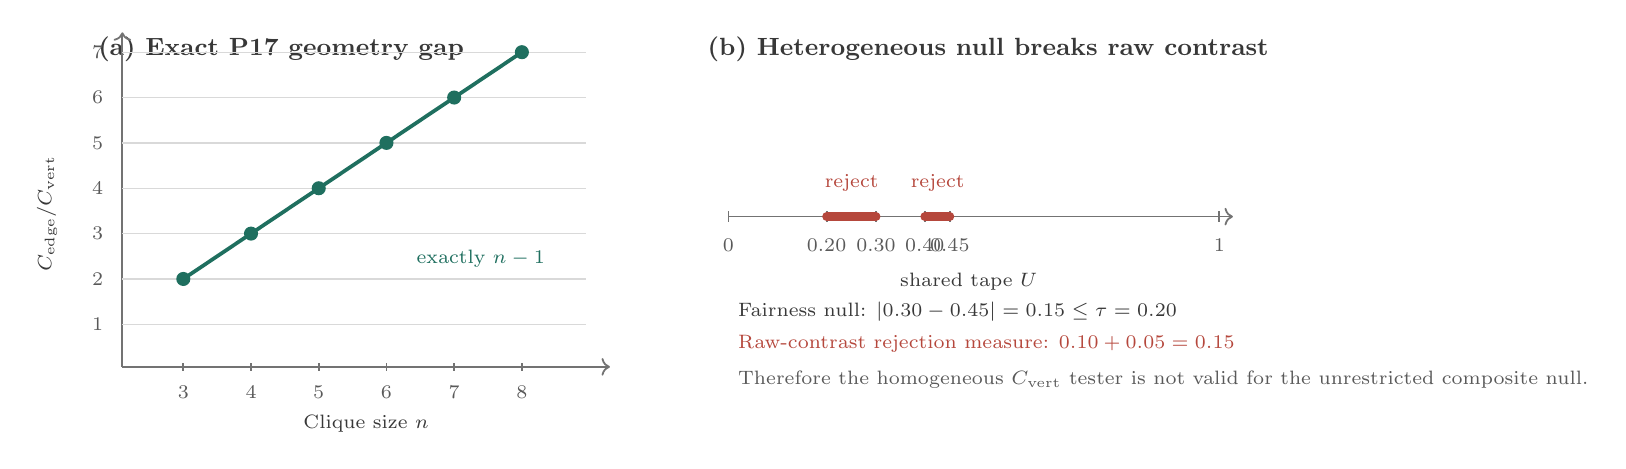
\begin{tikzpicture}[x=0.86cm,y=0.72cm,
  axis/.style={draw=black!55,line width=0.65pt},
  guide/.style={draw=black!15,line width=0.45pt},
  focalLine/.style={draw=focalteal,line width=1.35pt},
  riskLine/.style={draw=risktone,line width=3.2pt,line cap=round},
  pt/.style={circle,fill=focalteal,inner sep=1.8pt},
  lab/.style={font=\scriptsize,text=black!78},
  small/.style={font=\scriptsize,text=black!65}
]

% Panel (a): exact structural ratio.
\begin{scope}[shift={(0,0)}]
\node[lab,anchor=west,font=\small\bfseries] at (0,6.35) {(a) Exact P17 geometry gap};
\draw[axis,->] (0.5,0.75) -- (7.7,0.75);
\draw[axis,->] (0.5,0.75) -- (0.5,6.65);
\foreach \x/\n in {1.4/3,2.4/4,3.4/5,4.4/6,5.4/7,6.4/8}{
  \draw[axis] (\x,0.68)--(\x,0.82);
  \node[small,anchor=north] at (\x,0.58) {\n};
}
\foreach \y/\v in {1.5/1,2.3/2,3.1/3,3.9/4,4.7/5,5.5/6,6.3/7}{
  \draw[guide] (0.5,\y)--(7.35,\y);
  \node[small,anchor=east] at (0.36,\y) {\v};
}
\draw[focalLine] (1.4,2.3)--(2.4,3.1)--(3.4,3.9)--(4.4,4.7)--(5.4,5.5)--(6.4,6.3);
\foreach \x/\y in {1.4/2.3,2.4/3.1,3.4/3.9,4.4/4.7,5.4/5.5,6.4/6.3}{\node[pt] at (\x,\y) {};}
\node[lab,anchor=north] at (4.1,0.08) {Clique size $n$};
\node[lab,rotate=90,anchor=south] at (-0.32,3.45) {$C_{\rm edge}/C_{\rm vert}$};
\node[small,anchor=west,text=focalteal] at (4.7,2.65) {exactly $n-1$};
\end{scope}

% Panel (b): exact scope obstruction.
\begin{scope}[shift={(9.0,0)}]
\node[lab,anchor=west,font=\small\bfseries] at (0,6.35) {(b) Heterogeneous null breaks raw contrast};
\draw[axis,->] (0.45,3.4)--(7.9,3.4);
\foreach \x/\v in {0.45/0,1.90/0.20,2.63/0.30,3.35/0.40,3.72/0.45,7.70/1}{
  \draw[axis] (\x,3.31)--(\x,3.49);
  \node[small,anchor=north] at (\x,3.18) {\v};
}
\draw[riskLine] (1.90,3.4)--(2.63,3.4);
\draw[riskLine] (3.35,3.4)--(3.72,3.4);
\node[small,text=risktone,anchor=south] at (2.27,3.67) {reject};
\node[small,text=risktone,anchor=south] at (3.54,3.67) {reject};
\node[lab,anchor=north] at (4.0,2.58) {shared tape $U$};
\node[lab,anchor=west] at (0.45,1.72) {Fairness null: $|0.30-0.45|=0.15\le\tau=0.20$};
\node[lab,anchor=west,text=risktone] at (0.45,1.15) {Raw-contrast rejection measure: $0.10+0.05=0.15$};
\node[small,anchor=west] at (0.45,0.52) {Therefore the homogeneous $C_{\rm vert}$ tester is not valid for the unrestricted composite null.};
\end{scope}
\end{tikzpicture}
\caption{Exact deterministic P17 audit evidence.  (a) For clique $K_n$ with legal
replay groups equal to edges and unit costs, the witness geometry satisfies
$C_{\rm edge}/C_{\rm vert}=n-1$, giving an unbounded finite separation.
(b) The frozen heterogeneous fairness-preserving null triggers the homogeneous
raw-contrast predicate on two positive-measure tape intervals.  Both panels are
analytic consequences of the frozen fixtures, not Monte Carlo estimates.}
\label{fig:p17-audit}
\end{figure}

The final STOC submission will replace protocol-only entries in the experiment
ledger with measured stochastic summaries \emph{only after} a clean publication
run has been executed and archived with hashes and environment metadata. Until
then, the deterministic tables above are the only result tables we treat as
submission-facing evidence.
\section{Related Work and Novelty Boundary}
\label{sec:related}

\paragraph{Regression testing and change impact.}
Regression-test selection has long been studied as a way to reuse tests after
software modification \cite{RothermelHarrold1996,YooHarman2012}.  Code-based
change-impact analysis identifies which behavior may be affected by a change
\cite{LiSunLeungZhang2013}.  Our model treats sound impact information as side
information in a statistical query problem rather than proposing a new static
impact analysis.

\paragraph{Fairness testing and auditing.}
Themis established automated software fairness testing as a software-engineering
problem \cite{GalhotraBrunMeliou2017}.  Active fairness auditing gives theoretical
query-efficient algorithms for assessing fixed learned systems
\cite{YanZhang2022}.  We do not claim novelty for fairness testing or active
fairness auditing in isolation; our target is version-aware stochastic regression.

\paragraph{Property testing.}
Property testing provides the surrounding query-complexity framework.
Optimal monotonicity/Lipschitz testing on hypercubes and hypergrids is a canonical
example of graph-structured local checks determining a global property
\cite{ChakrabartySeshadhri2013}; tolerant testing can be much harder than ordinary
testing \cite{FischerFortnow2006}; and adaptivity hierarchies are known
\cite{CanonneGur2018}.  Our property and access model are different: observations
are stochastic executions of two evolving software versions, and old-version and
impact information are first-class inputs.

\paragraph{Adaptive information lower bounds.}
Adaptive fixed-confidence sampling is commonly analyzed through transcript-level
change-of-measure arguments.  We use the generic information-theoretic technique
of Kaufmann, Capp{\'e}, and Garivier \cite{KaufmannCappeGarivier2016} and
specialize the alternatives to counterfactual patch effects on graph edges.

\paragraph{Pairwise experimental design.}
Optimal design for selected pairwise mean comparisons has a substantial
statistical literature, including recent graph-based formulations
\cite{SinghSinghDavidov2025}.  Therefore the existence of a graph allocation
problem by itself is not a novelty claim.  The role of $\Psi$ here is as the core
information quantity arising from a regression-specific coupled execution oracle;
the intended contribution is the complete software-evolution query model and its
upper/lower complexity theory.

\paragraph{Incremental and probabilistic verification.}
Incremental verification seeks to reuse proof information from earlier program
versions \cite{YinEtAl2025}.  Couplings are a standard tool for relational
reasoning about probabilistic programs \cite{BartheEtAl2017}.  We combine the
version-reuse viewpoint with statistical testing of a fairness property rather
than attempting full formal equivalence verification.

\paragraph{Nondeterministic software testing.}
Flaky tests demonstrate that stochastic and environment-dependent execution is a
practical testing concern.  Recent OOPSLA work controls nondeterministic APIs to
expose flakiness \cite{YuanLinShi2026}.  Our theory abstracts such uncertainty as
an execution oracle and asks how it changes the fundamental cost of fairness
regression certification.


\bibliographystyle{alpha}
\bibliography{references}

\section*{AI Methodology}
ChatGPT (OpenAI) was used for substantive research ideation, literature triage,
proof exploration, code drafting, and manuscript drafting and structuring.  The human
authors are responsible for independently verifying every theorem, proof,
originality claim, citation, implementation, and final statement.  No generative
AI model, pretrained model, open-source model, or model API is a study subject,
research oracle or data source, or component of the experimental system analyzed
in this paper.

\end{document}
